\documentclass{article}

\usepackage{Paper}

\fancyhead[L]{Group 38}
\pdftitle{Tinkercad-exercise}
\setlength{\droptitle}{-2.5em}

% === TITLE ===
\title{\textbf{CAD exercises Block C3.1.2}}
\date{}

\geometry{
    a4paper,
    total={170mm, 257mm},   
    left=20mm,
    top=20mm,
    bottom=15mm
}

% === TEXT ===
\begin{document}
\maketitle
\thispagestyle{fancy}
\vspace{-2em}

\section*{Exercise 1: ``Your Name''}
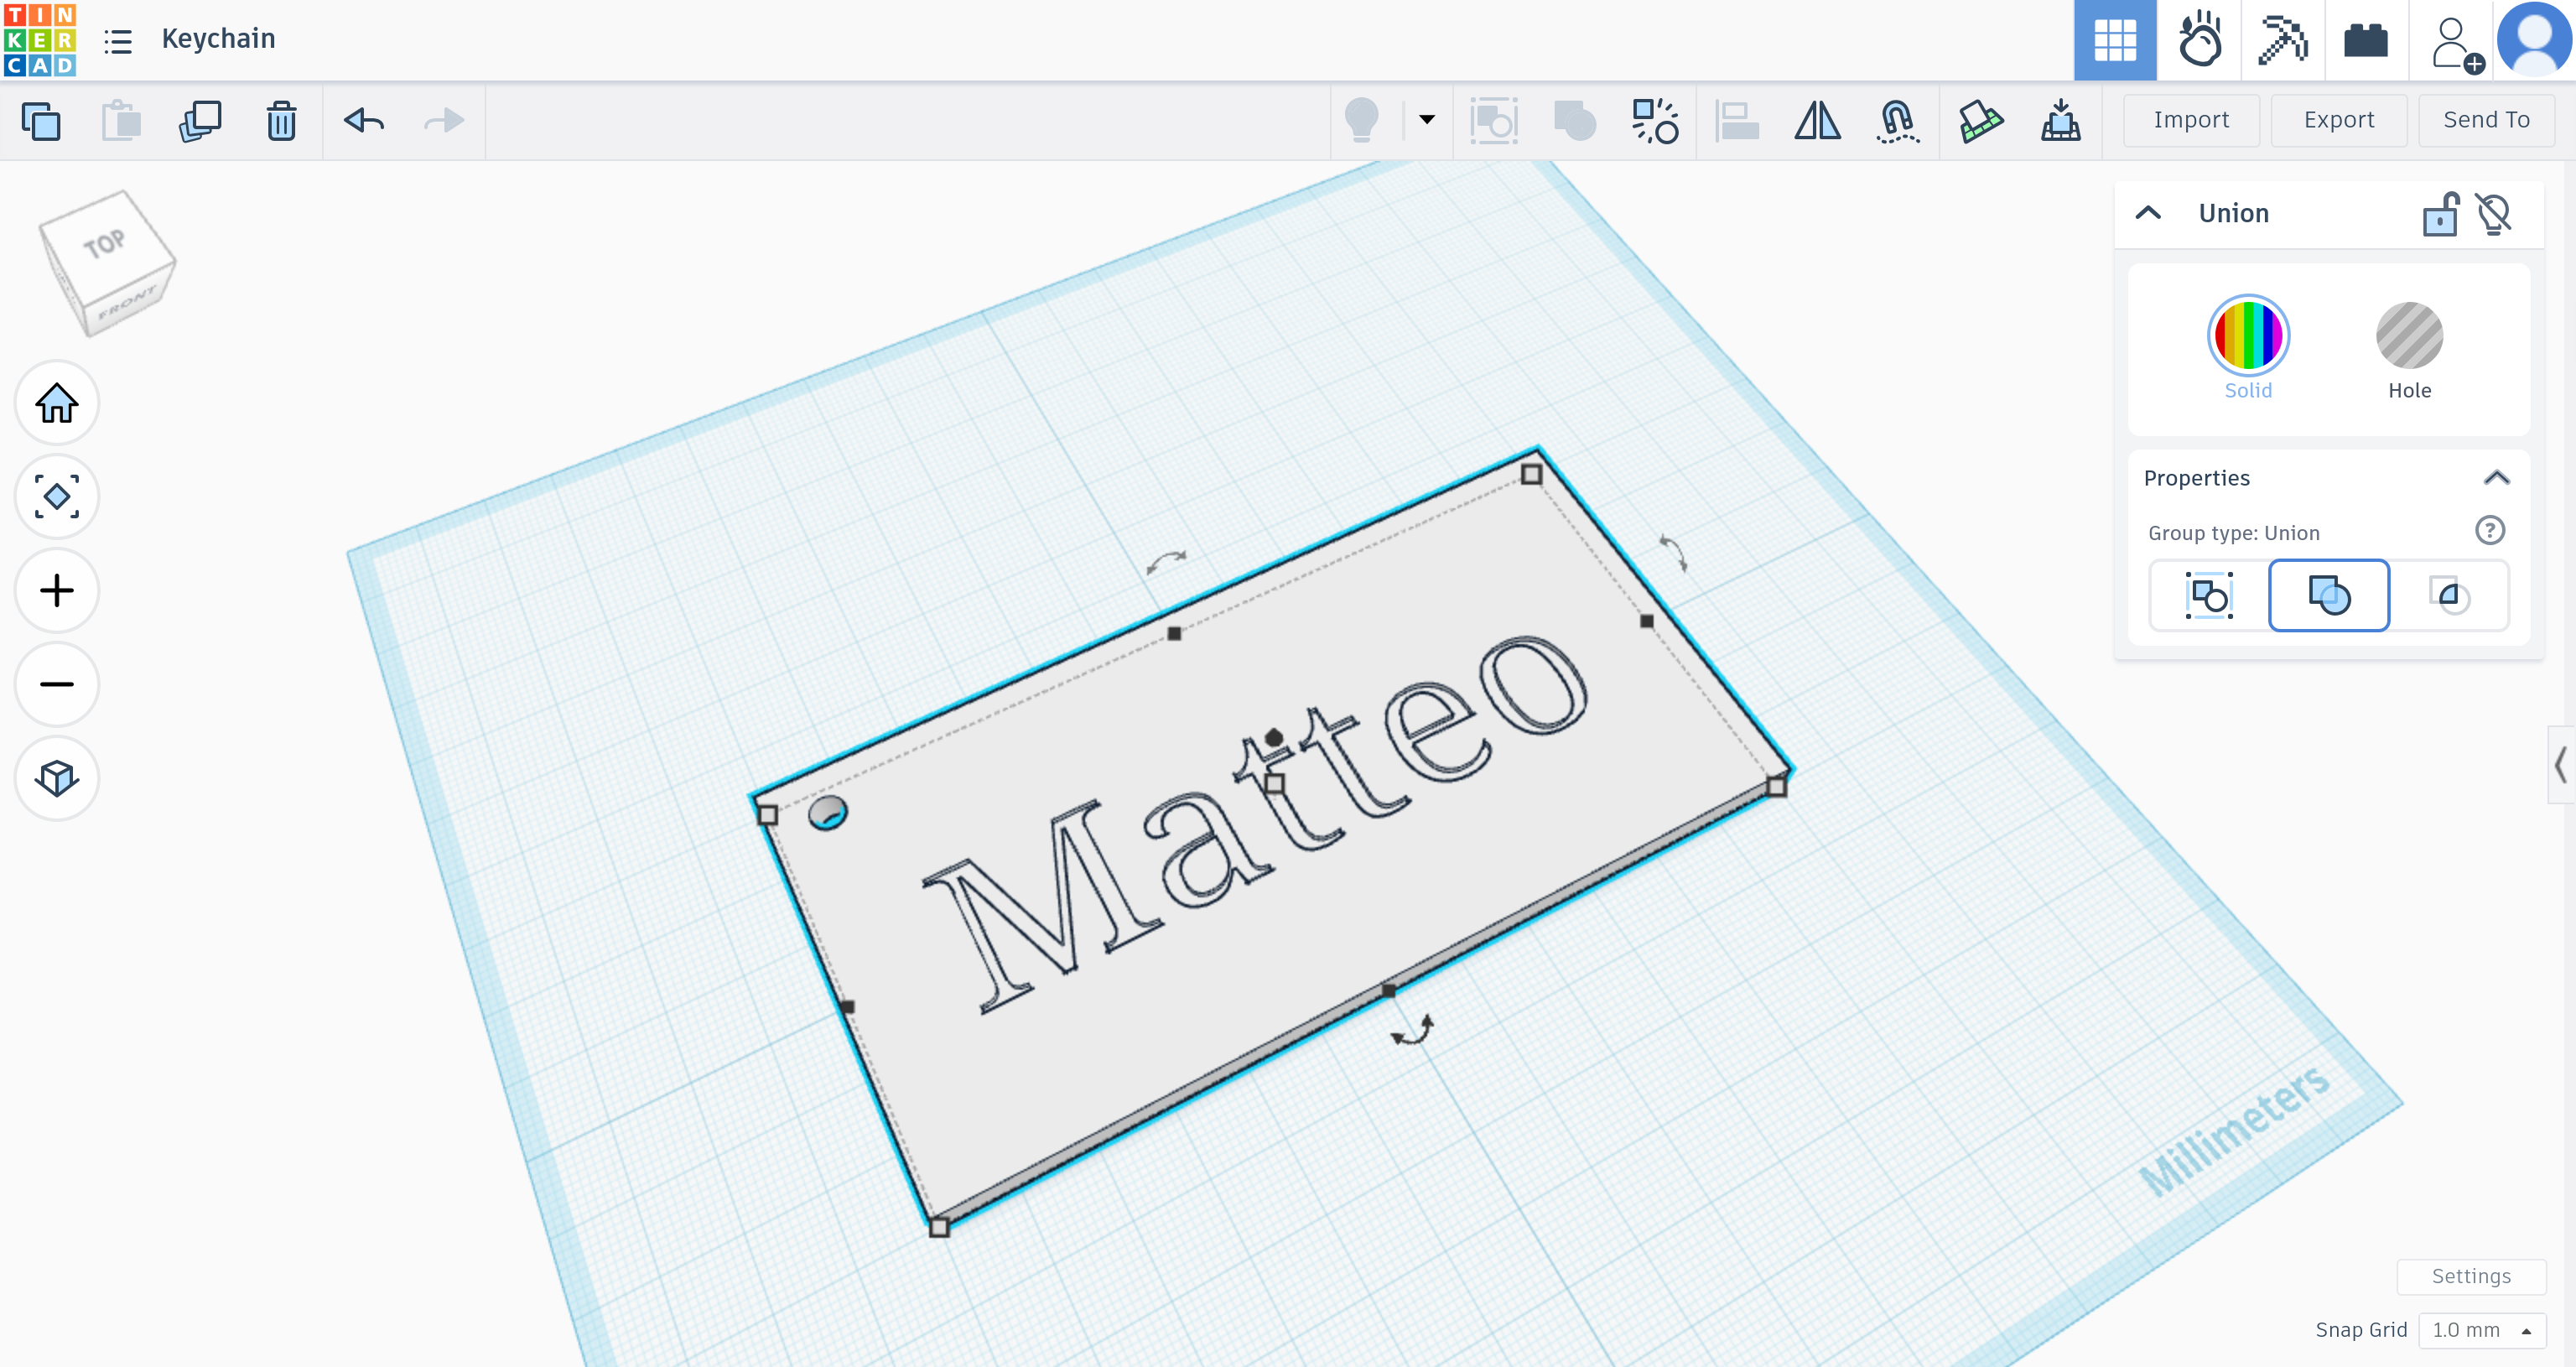
\includegraphics[\lw]{media/keychain.png}

The exercise already requires basic knowledge of how Tinkercad
works, such as creating an empty project, understanding the
difference between a solid and a hole block, and grouping multiple
blocks together. After going through the ``Lesson plan of CAD Block
C3.1.2'' in the ``All Daily Lesson Plans'' PDF provided in the
teacher documents, it becomes clear that nothing is really explained.
Moreover, most of the blocks are unfinished, so there is no relevant
information.

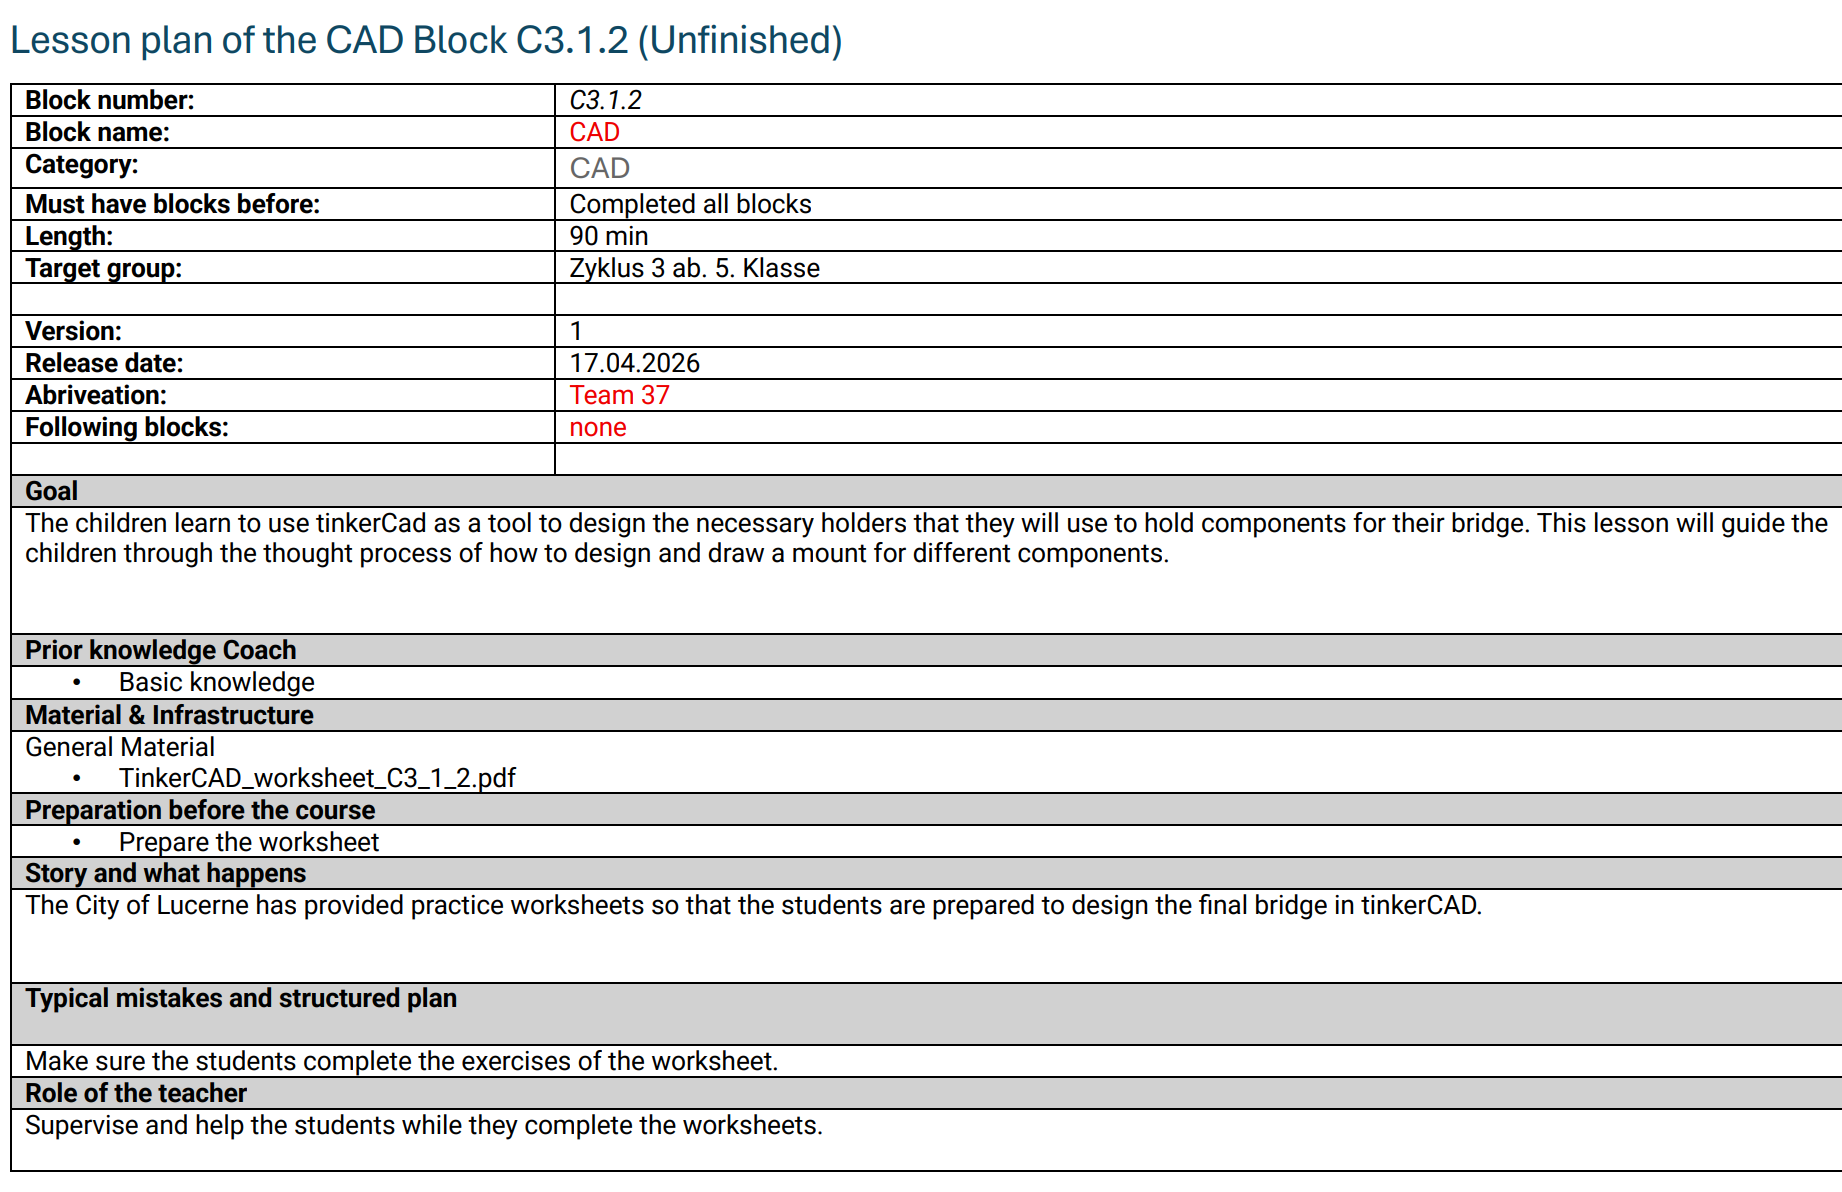
\includegraphics[\lw]{media/lesson.png}

\section*{Exercise 2: ``First Parts''}
There is no folder called ``For Engineers'', and the folder contains
two templates. The Tinkercad template does not have the same name as
the one stated in the exercise. Therefore, the folder should have been
structured better, and the naming should have been consistent with the
exercise.

The instructions for this exercise assume that the students already
know how to import files. Also, the imported block has to be rotated,
but the direction is not specified.

The instructions for the block to be
placed on top of the imported one do not state whether the hole should
be parallel or orthogonal to the holes on the bottom.

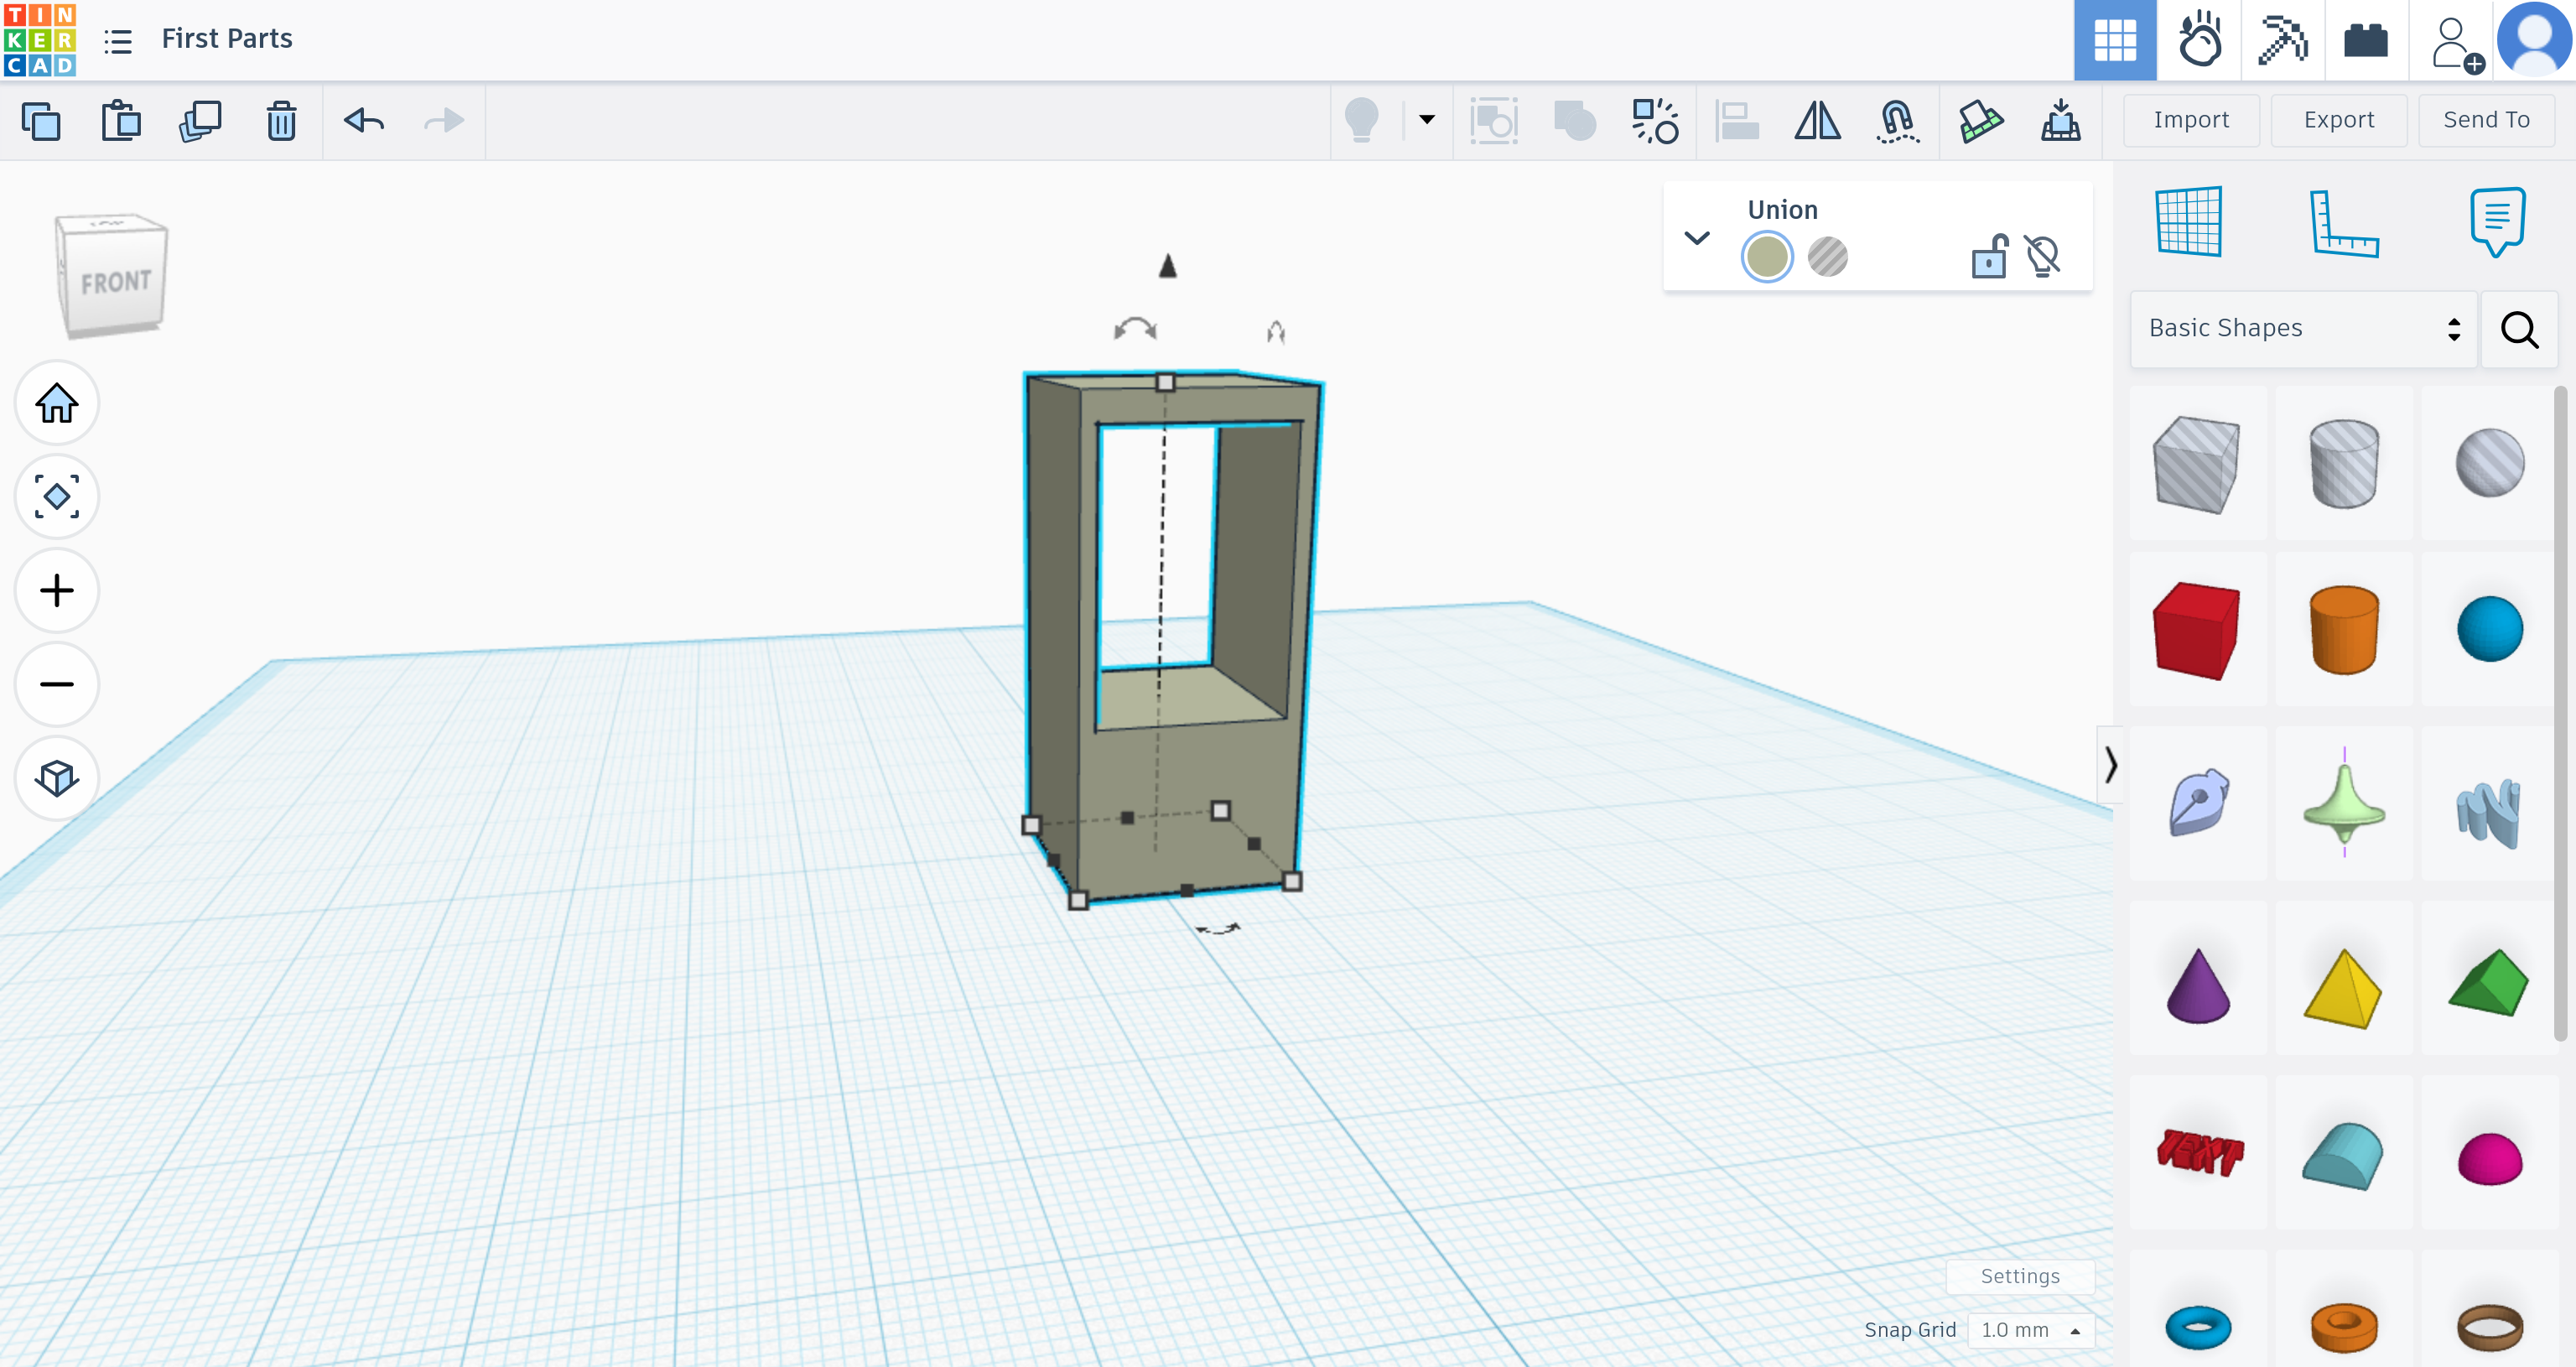
\includegraphics[\lw]{media/shape.png}






\end{document}
